\section{Computational Readiness}
\label{sec:readiness}

Single core performance comparison for both Hydro and M1: laptop, intel-16, \mira, \thet.

Say that all calculations are for leaf blocks only.

Emphasize effectively THREE steps per guardcell fill/synchronization. This is a big win. Hides the expense of communication with extra computation.

In testing, we used thread layout 1. In production, we use thread layout 2 to keep neighborhood threads together.

State cost of progenitor simulation .
% \subsection{Leadership Classification}
% Three-dimensional CCSN simulation is a quintessential {\it
%   Leadership-class} computational problem. The enormous resolution
% required, incredible number of time steps needed, and the challenging
% nature and variety of the physics involved make it so. Our proposed
% research requires Leadership computing because almost all of our requested allocation
% will be spent on one or a few simulations that run individually at the
% capability-scale ($\sim20\%$ of the system).

\subsection{Job Characterization \& Use of Requested Resources}
\label{sec:jobs}

We estimate the computational cost of our
simulations as follows.  We
assume an average shock radius of 200 km, inside of which the grid
will be refined to the maximum allowed level.
The maximum refinement level is radius dependent, establishing a grid in which the resolution increase logarithmically with radius.
Given the rate of this decrease in refinement with radius, the
average shock radius, and the finest possible grid spacing, $d
x_{\rm min}$, the time-averaged number of zones, $\bar N_{\rm zones}$,
can be estimated for each simulation.  Then, given the number of time
steps needed, $N_{\rm steps}$, the computational cost of a simulation
is $C = \alpha   \bar N_{\rm zones} N_{\rm steps}$,
where $\alpha$ is the use rate in units of core-hours per zone-step.
The number of time steps needed is determined by the
evolution time sought and the time step size: $N_{\rm steps} = t_{\rm
  max} / d t$.
The time step for an explicit integrator is $d t = a_{\rm CFL}\ {\rm min}[d x / (c_{\rm S} + v)]$, where $a_{\rm CFL}$ is a number less than one (typically 0.5 for MHD and 0.9 for M1 transport), $c_{\rm S}$ is the maximum signal speed and $v$ is the flow speed; this expression is computed locally for each zone.
For \sparkmone, the explicit neutrino transport approach makes the maximum signal speed the speed of light, which is about three times the sound speed in the center of the PNS and, thus, is always the limiting signal speed (even though we use a larger $a_{\rm CFL}$ for the M1 update).
The use rate, $\alpha$, is determined experimentally from actual simulations (see \S\ref{sec:performance}).  The time-averaged number of zones is estimated based on $d x_{\rm min}$, $\eta$, and the shock radius, behind which we assume maximal resolution.  Comparison to actual production simulations shows that our method for estimating the the computational cost is accurate.

The vast majority of our requested allocation will be expended on jobs at the Capability scale (20\% or more of the machine).
We take two approaches to achieving this: large monolithic jobs and packaged smaller jobs.
Specifically, the simulations proposed in Sections \ref{sec:Y1mrccsn}, \ref{sec:Y1progen}, \ref{sec:Y2late}, and \ref{sec:Y2progen} will be packaged into 8192-node jobs on \mira wherein each individual simulation is running on a sub-partition of 2048 nodes.


\subsection{Computational Approach}
\label{sec:approach}

Our primary tool for conducting the planned simulations will be the multi-physics, adaptive mesh refinement simulation framework, FLASH.
Specifically, we will primarily use our custom CCSN application \sparkmone that incorporates the new, high-performance \spark MHD solver \citep{Couch:2017} and our explicit two-moment neutrino transport solver \citep{OConnor:2015, OConnor:2015a}.
The code, now in its fourth major release version, has been continuously maintained, updated, extended, and modernized by the scientists at the Flash Center.
Additionally, as an acceptance and Early Science application on BG/Q {\it Mira}, FLASH has been exactingly tuned to take advantage of this impressive architecture (see \citet{Daley:2013esp}).
The block-structured, oct-tree adaptive mesh refinement in FLASH provides extreme flexibility and efficiency, particularly when combined with hybrid MPI/OpenMP parallelism.
Coupled with the neutrino physics and nuclear equation of state that we have already implemented, FLASH is a code ideally suited to tackling the magnetorotational CCSN problem.

FLASH contains a wide range of numeric solvers for solving
PDEs on block-structured AMR meshes. FLASH relies on the oct-tree
based PARAMESH library \citep{MacNeice:2000}. The proposed
simulations will solve the equations of hydrodynamics and
magnetohydrodynamics using an unsplit, explicit, finite-volume
Eulerian formulation (see Sec. \ref{sec:spark}).
FLASH utilizes hybrid MPI/OpenMP parallelism in order to make best use
of many-core architectures. The hydrodynamics/MHD
solvers, gravity solvers, and source terms have all been extended to
include support for thread-level parallelism via OpenMP.
FLASH writes output files using the HDF5 library. These files can be
read in directly and visualized in parallel using VisIt or yt
visualization software \citep{Turk:2011}.

Our \sparkmone application has been architected for performance.
Options such as reconstruction and Riemann solver are selected at compilation rather than runtime and are generally directly in-lined into the  calling routines in order to avoid function call overhead.
Aggressive use of Fortran array operations are employed and facilitate easy vectorization by the compiler.
In order to minimize cache misses, the reconstruction and flux calculation steps in \spark take place on auxiliary 1D ``pencil'' arrays that flatten an entire 1D ray of zones into a data structure that is contiguous in memory and much smaller than a one entire AMR block data structure.
All 1D reconstruction and flux computations are completed on these rays then before moving on to other rays, maximizing the number of operations performed per byte of data moved from memory.
This approach also facilitates efficient OpenMP threading wherein each thread operates on a collection of pencil arrays.
Communication is avoided during the multi-stage RK integration by filling and updating extra layers of guard, or halo, zones.
Thus, for WENO5, with a five-point stencil, and RK2 we require six guard zones per direction.
The M1 neutrino transport equations form a hyperbolic system of PDEs that is extremely similar to the MHD equations in structure and, thus, can be solved with similar methods.
Our implementation is a finite volume approach using second-order spatial reconstruction and third-order SSP RK time integration.
This approach makes full use of all six guard zones per direction and the high-order time integration increases stability, allowing M1-limited time steps up to CFL factors of $\gtrsim$0.9, greater than the typical MHD-limited CFL factor of $\sim$0.5.
This mitigates to some extent the increased number of time steps required by the explicit radiation transport approach and reduces the ratio of communication-to-calculation.


\subsubsection{Workflow Patterns}

The vast majority of the allocated time will be spent on production
simulations. We will utilize the Simulation management and analysis
system (Smaash, \citep{Hudson:2011}) that has been developed at the
Flash Center and ALCF explicitly for use in managing FLASH simulations
and data. Smaash monitors simulation progress, automatically sets-up
and schedules restarts, and moves data to tape archive. Smaash has an
intuitive web-based user interface and is built to maintain data
continuity and repeatability of simulations. Much of the data analysis
will be done {\it in-situ}.  Other analysis and visualization will be
conducted on the ALCF resource {\it Tukey} which is attached to the
same file system as {\it Mira}, obviating the need to move the data for
analysis.  We will use the QuickFlash library of C++ routines for
analyzing our data.  We will use VisIt and custom ALCF volume
rendering software for visualization.

\subsubsection{I/O}
Flash implements parallel HDF5 and collective I/O wherein a reduced
number of MPI ranks perform I/O to reduce the number of processes
accessing the file system at one time. The amount of time spent by
FLASH on I/O in a production simulation is typically less than five
percent of the overall run time. Use of the GLEAN library will
substantially reduce this time to negligible values as has been
demonstrated previously (see \citet{vishwanath2011}).

\subsubsection{Data Storage}
For the MRI simulation, the enormous number of zones is reflected
in large I/O files and storage requirements.  Each checkpoint file
will be 1 TB in size and plot files will be 300 GB.  We will produce
750 plot files and 75 checkpoints, which will require 300 TB of online
storage.  Following analysis and visualization, we will move the data
to permanent tape archive.
The M1 simulations will produce 150 GB checkpoints and 10 GB plot files.
We request a further 100 TB for storage of these data.
Disk space usage will be comparable in all three years of this project.




%Much of the allocation will be spent carrying out the one MRI-resolved simulation (\S\ref{sec:mriSim}).
%This simulation will be conducted on 8192 {\it Mira} nodes and will require 17 24-hour runs to complete.
%Due to the memory requirements of FLASH-MaRCC1 we will run this simulation using 8 MPI ranks/node and 8 OpenMP threads/rank.
%We estimate one restart per week, putting the time of completion in November.


\subsection{Parallel Performance}
\label{sec:performance}


FLASH has a long history of excellent scaling and performance on Leadership-class platforms.
We have benchmarked the performance and scaling of the FLASH-MaRCC1 application on {\it Mira}.
Our benchmarks use the full, production version of FLASH-MaRCC1, including MHD, self-gravity, AMR, neutrino leakage/M1 neutrino transport, and nuclear equation of state.
In Figure \ref{fig:scaling} we show the weak scaling on {\it Mira} for FLASH-MaRCC1 going up to 32,768 nodes (524k cores) for leakage and 8192 nodes (128k cores) for M1.
The leakage variant scales almost perfectly from 512 to 32,768 nodes.
Our M1 version of FLASH does not scale as efficiently because it requires a great deal more communication since the M1 calculation needs over 150 extra grid variables than the leakage does.
We are working on improvements to the communication efficiency for the M1 variant that should increase scaling efficiency prior to the start of the INCITE allocation.
As is to be expected, IO does not scale perfectly.
Despite the exponential growth in the time required for IO, it is still only a small fraction ($\sim5\%$) of the total runtime during production simulations since IO occurs so infrequently.
We also plot in Fig. \ref{fig:scaling} the strong scaling and thread-to-thread speedup for FLASH-MaRCC1.
Both are quite acceptable for capability-level production simulations.


In order to gauge our performance, we have benchmarked FLASH against another comparable compressible MHD code, Athena (v4.2).\footnote{This comparison is only included because there was confusion on the part of at least one reviewer during the review of our INCITE proposal last year.
Concerns were raised over the apparent inefficiency of FLASH based on our performance metrics.
The reviewer accused FLASH of being ``10$\times$'' slower than other comparable MHD codes without giving an actual reference.
Of course this was a major shock and concern for us.
Thus, we present this comparison with Athena, an excellent MHD code that is well-known as being highly efficient and fast.
}
We use the common Field Loop Advection problem described in \citet{Gardiner:2008dh} and \citet{Lee:2009kq}, which is a standard test problem packaged with the release versions of both codes.  We use a fixed-resolution grid for these tests and the same parameters across all three codes.

%We first tested the performance on a 4-core laptop using a grid of 32x32x64 zones.  Compared to FLASH, Pluto is 2.9x faster and Athena is 4x faster.  This is a significant inefficiency that we have been working to alleviate.  We have already optimized the non-MHD unsplit solver in FLASH yielding a 2.5x speedup in 3D performance. Consumer grade hardware, however, exhibits very different performance characteristics than leadership-scale hardware.  A great deal of effort has gone into optimizing FLASH for the BG/Q architecture and FLASH has been tested and developed on BG/Q since the start of the Mira Early Science Program.


We have conducted the Field Loop Advection problem on BG/Q Cetus using both FLASH and Athena.
For all tests on Cetus, we use 4096 zones per MPI ranks and the same fixed-resolution grid.
On Cetus, we use 16 MPI ranks per node.
Athena utilizes only MPI parallelism without any support for threading.
Given the unique architecture of BG/Q, which allows for up to 4 hardware threads per core, this means that Athena cannot utilize the full power of this architecture.
We run two Athena benchmarks on Cetus:  in the first we use 1 node (16 cores) and a grid of 32x32x64.
In the second Athena run we use 512 nodes (8192 cores) and a grid of 256x256x512.
We run several comparable FLASH benchmarks using different OMP thread counts (1 and 4).
The results of our benchmarks are shown in Table \ref{table:perf}.
The performance numbers show the zone-steps per cpu-second (in parentheses) and MSU per zone-step (first number).


\begin{deluxetable}{llll}
\tablecolumns{4}
\tabletypesize{\scriptsize}
\tablecaption{
Single-thread performance comparisons on different hardware platforms in units of core-hours/zone-step (zone-step/core-second).
\label{table:perf}
}
\tablewidth{0pt}
\tablehead{
\colhead{ } &
\colhead{FieldLoop \spark} &
\colhead{FieldLoop USM-CT} &
\colhead{CCSN \sparkmone}
}
\startdata
  Intel Core i7 (I7-6567U) & 2.15e-09 (129,075) & 7.09e-09 (39,173) & 1.80e-07 (1545) \\
  Intel Xeon E5-2680v4     & 1.76e-09 (157,808) & 4.42e-09 (62,779) & 1.05e-07 (2658) \\
  IBM BG/Q A2              & 2.58e-08 (10,787)  & 6.58e-08 (4221)   & 2.75e-06 (103) \\
  Intel KNL                & 7.41e-09 (37,494)  & 2.81e-08 (9881)   & 7.00e-07 (397)
\enddata
\end{deluxetable}

As shown, we find that the 1-node performance of FLASH is very similar to that of Athena on BG/Q, that is when FLASH is run in single-thread mode.  For multiple thread configurations FLASH outperforms Athena.
Leveraging the full threading abilities of BG/Q, we see that FLASH is about 2x faster than Athena.
Also clear from the 512-node benchmarks, FLASH shows more efficient weak scaling than Athena.  As we demonstrate above, FLASH scales to nearly the entire Mira platform with extreme efficiency.

The performance of FLASH for the field loop advection problem is significantly better than for the full MaRCC1 application (see Fig. \ref{fig:scaling}) for several reasons.
In MaRCC1 we use WENO-5 instead of PPM, a complex microphysical tabular EOS, self-gravity, neutrino physics, extensive on-the-fly data analytics, and I/O.
This all serves to approximately double the per zone-step cost of the MaRCC1 application as compared with the simple Field Loop Advection test.
We further emphasize that while comparable performance for the Field Loop Advection test may be obtained with Athena, Athena lacks the long list of capabilities required to carry out the research we propose (i.e., AMR, nuclear EOS, neutrino physics).

\subsection{Developmental Work}

\subsection{Development plan for next-generation systems}


%\begin{wrapfigure}[41]{r}{3.25in}
\begin{figure}
  \begin{tabular}{r}
    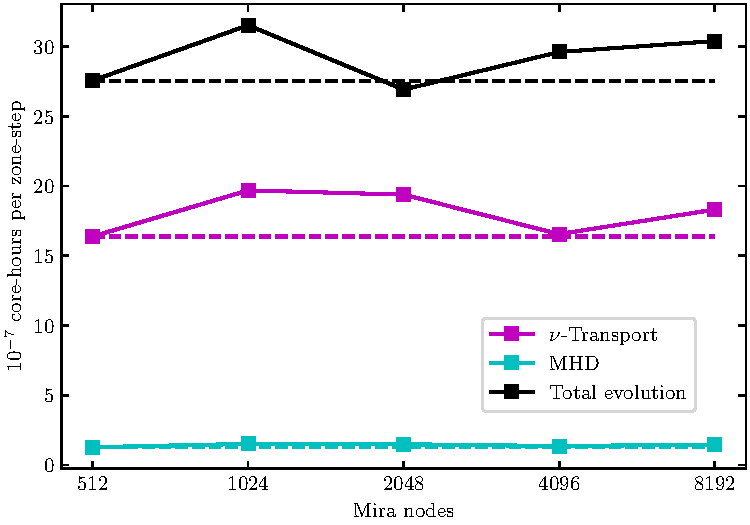
\includegraphics[width=3.25in]{figs/wkScaleSparkM1} \\
    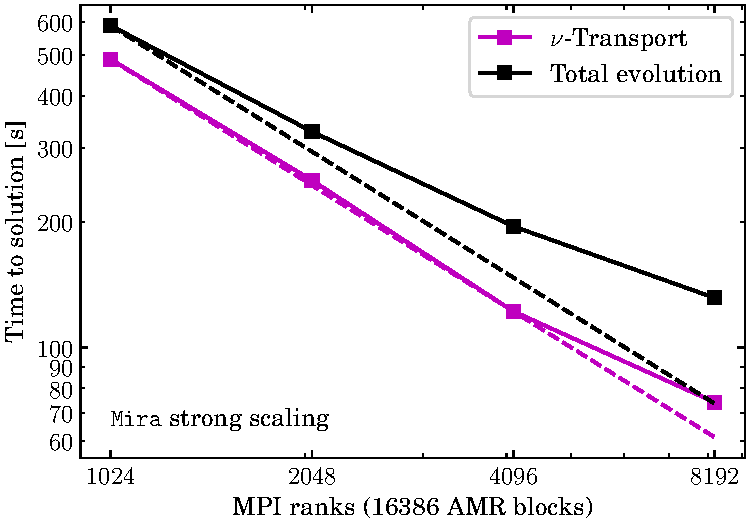
\includegraphics[width=3.25in]{figs/strScaleSparkM1} \\
    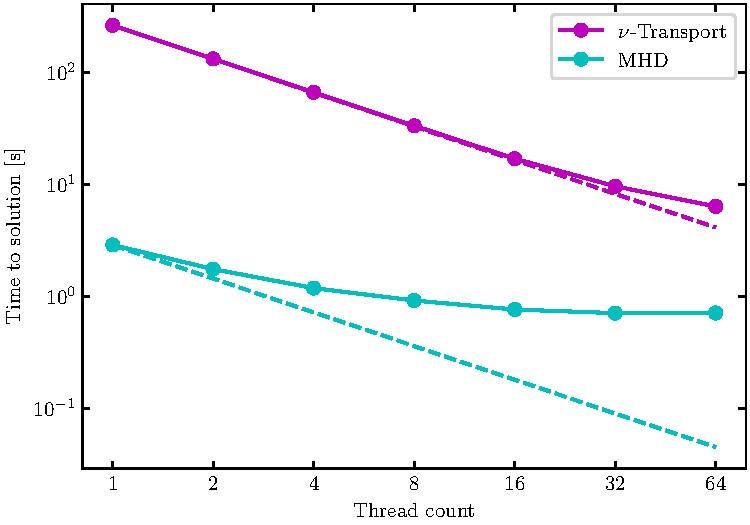
\includegraphics[width=3.25in]{figs/thrdSpeedupSparkM1}
  \end{tabular}
  \caption{Weak scaling (top), strong scaling (middle), and threading
  speedup (bottom) of FLASH-MaRCC1 on {\it Mira}.  Note that for this configuration, use of 8 threads can result in a maximum theoretical speedup of 4x.}
  \label{fig:scaling}
\end{figure}
%\end{wrapfigure}
